\documentclass[12pt, a4paper]{article}

\usepackage[utf8]{inputenc}
\usepackage[T1]{fontenc}
\usepackage[russian]{babel}
\usepackage[oglav,spisok,boldsect, figwhole]{./style/fn2kursstyle1}
\graphicspath{{./style/}{./figures/}}
%\usepackage{float}%"Плавающие" картинки
\usepackage{multirow}
\usepackage{subcaption}
\usepackage{float}%"Плавающие" картинки
%Римские цифры
\newcommand{\RomanNumeralCaps}[1]
{\MakeUppercase{\romannumeral #1}}

\usepackage{enumitem} 
\usepackage{amsmath}
\usepackage{comment}
\usepackage{makecell}

%Параметры титульника
\title{Численное решение краевых задач для одномерного уравнения теплопроводности}
\group{ФН2-62Б}
\author{З.И.~Абрамов, Г.А.~Швецов}
\supervisor{С.А.~Конев}
\date{2023}
\begin{document}
	\newcommand{\pl}{\partial}
	\maketitle
	
	\tableofcontents
	
	\newpage
	
	\section{Контрольные вопросы}
	\begin{enumerate}
		\item \textit{Дайте определения терминам: корректно поставленная задача, понятие аппроксимации дифференциальной задачи разностной схемой, порядок аппроксимации, однородная схема, консервативная схема, монотонная схема, устойчивая разностная схема (условно/абсолютно), сходимость.}
		\smallskip
		
		\textbf{Задача} называется \textbf{корректно поставленной}, если ее решение существует, единственно и непрерывно зависит от входных данных. Если же не выполнено хотя бы одно из этих условий, то \textbf{задача} называется \textbf{некорректно поставленной}.
		
		Рассмотрим точную задачу
		\[
		A u = f \text{ в } G, \quad R u = \mu \text{ на } \Gamma
		\]
		и <<заменяющую>> ее разностную схему
		\[
		A_h y = \varphi \text{ в } G_h, \quad R_h u = \nu \text{ на } \Gamma_h.
		\]
		
		В этом случае
		\[
		\psi_h = (\varphi - f_h) + ((A v)_h - A_h v_h), \quad \chi_h = (\nu - \mu_h) + ((R v)_h - R_h v_h) \text{ ---}
		\]
		погрешности аппроксимации разностной задачи (для общего случая произвольной функции $v$) в $G_h$ и на $\Gamma_h$ соответственно.
		
		\textbf{Разностная схема аппроксимирует} исходную \textbf{задачу}, если $\|\psi_h\|_\psi \rightarrow 0$, $\|\chi_h\|_\chi \rightarrow 0$ при $h \rightarrow 0$; аппроксимация имеет $p$-й порядок ($p > 0$), если $\|\psi_h\|_\psi \brop= O(h^p)$, $\|\chi_h\|_\chi = O(h^p)$ при $h \rightarrow 0$.
		% Как надо интерпретировать объект h в случае схемы для многомерного уравнения?
		В многомерном случае под $h$ можно понимать вектор из шагов сетки (в двумерном случае вектор из шага по времени $\tau$ и пространству $h$), а под $p$ --- мультииндекс.
		
		\textbf{Разностные схемы}, в которых расчет ведется по одним формулам и на одном шаблоне во всех узлах сетки без какого-то специального выделения имеющихся особенностей, называются \textbf{однородными}.
		
		\textbf{Разностные схемы} называют \textbf{консервативными} (дивергентыми), если их решение удовлетворяет дискретному аналогу закону сохранения (баланса), присущему исходной задаче. В противном случае схему называют \textbf{неконсервативной}, или дисбалансной.
		
		\textbf{Схемы}, решение которых удовлетворяет принципу максимума или сохраняет пространственную монотонность (в одномерном случае) при условии, что соответствующие свойства справедливы для исходных задач, называются \textbf{монотонными}.
		
		Пусть $y^I$, $y^{II}$ --- решения двух разностных задач с одинаковым оператором, соответствующие правым частям $\varphi^I$, $\varphi^{II}$ и граничным условиям $\nu^I$, $\nu^{II}$.
		
		\textbf{Разностную схему} называют \textbf{устойчивой}, если решение уравнений разностной схемы непрерывно зависит от входных данных и эта зависимость равномерна по $h$, т.е.
		\[
		\forall\varepsilon \; \exists\delta(\varepsilon)>0: \| \varphi^I - \varphi^{II}\|_\varphi < \delta, \; \|\nu^I - \nu^{II}\|_\nu < \delta \Rightarrow \|y^I-y^{II}\|_Y < \varepsilon.
		\]
		
		% В определении непрерывности решения схемы от входных данных — предполагается зависимость 𝛿 от h, или нет?
		\looser{-0.01}{При этом отдельно можно отметить, что значение $\delta$ не зависит от шага сетки $h$.}
		
		В случае нескольких независимых переменных \textbf{устойчивость} называют \textbf{безусловной} (или абсолютной), если устойчивость имеет место для любого соотношения шагов, и \textbf{условной} в противном случае. 
		
		Разностное решение y сходится к решению $u$ точной задачи, если $\|y-p_h u\|_Y \rightarrow 0$ при $h \rightarrow 0$. Говорят, что имеет место \textbf{сходимость} с $p$-м ($p > 0$) порядком, если $\|y-p_h u\|_Y = O(h^p)$ при $h \rightarrow 0$.
		
		\item \textit{Какие из рассмотренных схем являются абсолютно устойчивыми? Какая из рассмотренных схем позволяет вести расчеты с более крупным шагом по времени?}
		\smallskip
		
		Для исследования на устойчивость применим принцип замороженных коэффициентов, т.е. примем, что $a_i = a_{i+1} = a$. Тогда смешанная схема примет следующий вид:
		\[
		c\rho\frac{y_i^{j+1}-y_i^j}\tau = \sigma a \frac{y_{i+1}^{j+1} - 2y_i^{j+1} + y_{i-1}^{j+1}}{h^2} + (1-\sigma) a \frac{y_{i+1}^j - 2y_i^j + y_{i-1}^j}{h^2}.
		\]
		
		Далее воспользуемся методом разделения переменных и разложим $y$ по собственным функциям оператора второй разностной производной, т.е.
		\[
		y_i^j = \sum_{k=1}^{n-1} c_k^j \mu_{k, i}, \quad \mu_{k, \overline{x} x} + \lambda_k^2 \mu_k = 0, \quad \lambda_k = \frac4{h^2} \sin \frac{\pi k h}{2l}.
		\]
		
		Здесь $\mu_{k, i} = \sin \sfrac{\pi k i h}l$, $k = \overline{1, n-1}$ --- собственные функции разностной производной. Подставляя в схему, получаем следующее выражение:
		\begin{eqnarray*}
			& c\rho \sum\limits_{k=1}^{n-1}\dfrac{c_k^{j+1}-c_k^j}\tau \mu_{k, i} = a \sum\limits_{k=1}^{n-1} (-\lambda_k^2 \sigma c_k^{j+1} \mu_{k, i} ) + a \sum\limits_{k=1}^{n-1} (-\lambda_k^2 (1-\sigma) c_k^j \mu_{k, i} ), \\
			& \sum\limits_{k=1}^{n-1} \left(c\rho \dfrac{c_k^{j+1}-c_k^j}\tau\right) \mu_{k, i} = \sum\limits_{k=1}^{n-1} -\lambda_k^2 a(\sigma c_k^{j+1} + (1-\sigma) c_k^j) \mu_{k, i}.
		\end{eqnarray*}
		
		В силу ортогональности функций $\mu_k$ для любого $k = \overline{1, n-1}$ должно выполнятся равенство
		\[
		c\rho \dfrac{c_k^{j+1}-c_k^j}\tau = -\lambda_k^2 a(\sigma c_k^{j+1} + (1-\sigma) c_k^j).
		\]
		
		Из этого следует, что коэффициент у $j$-й гармоники меняется в
		\[
		\varrho_j = \frac{1 - \lambda_k^2 \tilde{a}(1-\sigma)}{1+\lambda_k^2 \tilde{a} \sigma}, \quad \textrm{где } \tilde{a} = \frac{a \tau}{c\rho}.
		\]
		
		Для устойчивости требуется, чтобы $|\varrho_j| \le 1$. Т.к. знаменатель положителен, то неравенство записывается как
		\[
		- (1+\lambda_k^2 \tilde{a} \sigma) \le 1 - \lambda_k^2 \tilde{a} + \lambda_k^2 \tilde{a} \sigma \le 1+\lambda_k^2 \tilde{a} \sigma.
		\]
		
		Заметим, что правая часть неравенства автоматически выполнена. Тогда получаем, что
		\[
		2 \lambda_k^2 \tilde{a} \sigma \ge \lambda_k^2 \tilde{a} - 2, \qquad \sigma \ge \frac12 - \frac1{\lambda_k^2 \tilde{a}}, \qquad \sigma \ge \frac12 - \frac{c\rho h^2}{4 a \tau}.
		\]
		
		Данное неравенство должно выполнятся при любых $a$. Таким образом, условие устойчивости записывается как
		\[
		\sigma \ge \frac12 - \frac{c\rho h^2}{4 a_{\max} \tau}.
		\]
		
		Из него же следует, что схема абсолютно устойчива при $\sigma \ge \sfrac12$.
		
		% Пожалуйста, обоснуйте тактику «замораживания» коэффициента?
		В обоснование принципа замороженных коэффициентов можно привести следующее рассуждение на эвристическом уровне строгости. При измельчении сетки коэффициент $a(x, t)$ в окрестности точки $(x^*, t^*)$ за любое фиксированное число шагов сетки длины $h$ по пространству и длины $\tau$ по времени ввиду непрерывности функции $a(x, t)$ меняется все меньше и все меньше отличается от значения $a(x^*, t^*)$. Поэтому при мелкой сетке возмущения, наложенные на решение задачи с переменным коэффициентом в момент времени $t = t^*$ в окрестности точки $x = x^*$ развиваются примерно так же, как для задачи с постоянным коэффициентом, равным $a(x^*, t^*)$\cite{godunov}.
		
		Также принцип можно обосновать тем, что решение должно быть устойчивым при любом диапазоне значений $a$, даже при самом "плохом". Поэтому можно исходить из того, что мы выбрали то самое плохое значение и исследовать схему при нем. В конце вывода условия мы определили, что таким "плохим" значением является максимальное значение функции $a$.
		
		% старое, оставил на всякий случай
		\begin{comment}
			В случае $a_i = \sfrac{K(x_i)+K(x_{i-1})}{2}$ погрешность аппроксимации имеет следующий вид (получено с использованием Wolfram Mathematica):
			\begin{multline*}
				\psi_h = \frac12 \tau(1-2\sigma) (K' u^{(1,1)} + K u^{(2,1)}) - \\
				- \frac1{12} h^2 \left(2 K''' u^{(1,0)} + 3 K'' u^{(2,0)} + 2 K' u^{(3,0)} + K u^{(4,0)}\right) + O(h^3 + \tau^2)
			\end{multline*}
			
			Заметим, что коэффициент при $h^2$ не зависит от $\sigma$. Также можно заметить, что при $\sigma = \sfrac12$ коэффициент при $\tau$ обнуляется и порядок схемы становится равным $O(h^2 + \tau^2)$. Т.е. использование схемы с $\sigma=\sfrac12$ позволяет вести расчеты с более крупным шагом.
		\end{comment}
		
		Используя Wolfram Mathematica, можно достаточно легко найти порядок аппроксимации $\psi_h$. При наложении условий, полученных в третьем контрольном вопросе, и при применении описанного там же процесса приходим к тому, что
		\[
		\psi_h = \left[ \left( K'(x_i) - 2\sigma\frac{a_{i+1}-a_i}h \right) \frac{u_{i, xt}^j}2 + \left(K(x_i) - \sigma(a_i + a_{i+1})\right) \frac{u_{i, xxt}^j}2\right]\tau + O(h^2 + \tau^2).
		\]
		
		Заметим, что в случае наложенных условиях на $a_i$ только при $\sigma = \sfrac12$ порядок схемы по времени становится равным 2. Таким образом, симметричная схема позволяет вести расчеты с более крупным шагом.
		
		\item \textit{Будет ли смешанная схема (2.15) иметь второй порядок аппроксимации при\\ $a_i=\sfrac{2K(x_i)K(x_{i-1})}{K(x_i)+K(x_{i-1})}$?}
		\smallskip
		
		Найдем порядок аппроксимации смешанной схемы в случае произвольного $a_i$:
		\begin{multline*}
			\psi_h = c \rho \frac{u_i^{j+1}-u_i^j}\tau - \frac1h\Bigg[\sigma\left(a_{i+1}\frac{u_{i+1}^{j+1}-u_i^{j+1}}h - a_i\frac{u_i^{j+1}-u_{i-1}^{j+1}}h\right) + \\
			%
			+(1-\sigma)\left(a_{i+1}\frac{u_{i+1}^j - u_i^j}h - a_i \frac{u_i^j - u_{i-1}^j}h\right)\Bigg] = c \rho \frac{u_i^{j+1}-u_i^j}\tau - \frac1{h^2} \cdot \\
			%
			\Big[\sigma \left(a_{i+1}(u_{i+1}^{j+1}-u_i^{j+1}) - a_i(u_i^{j+1}-u_{i-1}^{j+1})\right) + (1-\sigma)\left(a_{i+1}(u_{i+1}^j - u_i^j) - a_i (u_i^j - u_{i-1}^j)\right)\Big].
		\end{multline*}
		
		Используя замену $\tau \rightarrow \alpha \tau$, $h \rightarrow \alpha h$ в аргументах функции решения $u$, исходное уравнение теплопроводности и систему компьютерной алгебры Wolfram Mathematica, можно разложить $\psi_h$ в ряд по $\alpha$ в нуле и взять значение $\alpha = 1$. Таким образом можно построить разложение по $h$ и $\tau$. Приведем результат:
		\begin{multline*}
			\psi_h = \left[-\left(\frac{a_{i+1}-a_i}h - K'(x_i)\right) u_{i, x}^j - \left(\frac{a_{i+1} - a_i}2 - K(x_i)\right) u_{i, xx}^j\right] + \\
			%
			+ \left[\frac16 (a_i - a_{i+1}) u_{i, xxx}^j\right]h + O(\tau) + O(h^2) + O(h \tau).
		\end{multline*}
		
		Т.к. $O(h\tau) = O(h^2 + \tau^2)$, то для второго порядка аппроксимации по пространству достаточно выполнения следующий условий:
		\[
		\begin{cases}
			\dfrac{a_{i+1}-a_i}h = K'(x_i) + O(h^2), \\
			\dfrac{a_{i+1} - a_i}2 = K(x_i) + O(h^2), \\
			a_i - a_{i+1} = O(h).
		\end{cases}
		\]
		
		Заметим, что из выполнения первого условия автоматически следует выполнение третье. В итоге получаем, что достаточные условия для второго порядка по пространству смешанной схемы такие же, как и у схемы с параметром $\sigma = 1$:
		\[
		\begin{cases}
			\dfrac{a_{i+1}-a_i}h = K'(x_i) + O(h^2), \\
			\dfrac{a_{i+1} - a_i}2 = K(x_i) + O(h^2).
		\end{cases}
		\]
		
		Применяя, к примеру, команду Series системы Wolfram Mathematica, нетрудно убедиться, что $a_i=\sfrac{2K(x_i)K(x_{i-1})}{K(x_i)+K(x_{i-1})}$ удовлетворяет полученным требованиям. Таким образом, при использовании указанных $a_i$ численная схема будет обладать вторым порядком аппроксимации по пространству.
		
		\item \textit{Какие методы (способы) построения разностной аппроксимации граничных условий (2.5), (2.6) с порядком точности $O(\tau+h^2)$, $O(\tau^2+h^2)$ и $O(\tau^2+h)$ вы знаете?}
		\smallskip
		
		% TODO расписать получше
		
		Условия (2.5) и (2.6) имеют вид:
		\[
		-K(u, 0) \frac{\partial u}{\partial x}\Bigg|_{(0,t)} = P(t) \quad \text{и} \quad K(u, L) \frac{\partial u}{\partial x}\Bigg|_{(L,t)} = P(t).
		\]
		
		Граничные условия можно аппроксимировать следующими способами.
		
		\textbf{Метод разностной аппроксимации} заключается в том, что каждая производная, входящая в дифференциальное уравнение и краевые условия, заменяется каким-либо разностным (включающим только узлы шаблона). Для достижения нужного порядка аппроксимации необходимо использовать разностные аналоги производных соответствующего порядка. Например, в граничных условиях, указанных выше, можно заменить производную на ее разностный аналог в виде производной назад и получить первый порядок по пространству и бесконечный по времени. Также можно применить другие разностные производные, например, получаемые при выводе методов Адамса --- Башфорта.
		
		\textbf{Интегро-интерполяционный метод.} При использовании данного метода дифференциальное уравнение интегрируется по ячейке и приводят к интегральной форме, соответствующей физическому закону сохранения. Приближенно вычисляя полученные интегралы по каким-либо квадратурным формулам, составляют разностную схему. Именно выбор квадратурных формул и ячейки интегрирования определяют порядок аппроксимации численной схемы. Например, в методическом пособии при выводе схемы с весами для достижения второго порядка по пространству используется квадратурная формула центральных прямоугольников, имеющая как раз второй порядок.
		
		\textbf{Метод неопределенных коэффициентов} заключается в том, что в качестве разностной схемы берут линейную комбинацию значений разностного решения в узлах заданного шаблона. Коэффициенты этой линейной комбинации определяют из условия, чтобы невязка схемы имела необходимый порядок малости относительно $\tau$ и $h$.
		
		Для уравнения теплопроводности $u_t = k u_{xx}$ можно искать разностную схему в следующем виде:
		\[
		\alpha\hat y_{n-1}+\beta\hat y_n+\gamma\hat y_{n+1}+\delta y_n=0.
		\]
		
		Разложим выражение и вычтем его схему выше:
		\begin{multline*}
			\psi_h = u_t - k u_{xx} - (\alpha+\beta+\gamma+\delta)u + \tau \delta u_t + (\alpha-\gamma)h u_x - \\
			- \frac12(\alpha+\gamma)h u_{xx} + \delta O(\tau^2) + (\alpha-\gamma) O(h^3) + \dots
		\end{multline*}
		
		Таким образом, для получения второго порядка по времени и третьего по пространству надо положить
		\[
		\alpha+\beta+\gamma+\delta = 0, \quad \tau\delta = -1, \quad \alpha - \gamma = 0, \quad \frac12(\alpha+\gamma)h^2 = -k.
		\]
		
		Решив полученные уравнения, находим коэффициенты схемы.
		
		\textbf{Метод фиктивной точки} заключается в добавлении дополнительного узла вне области сетки. Приведем пример для уравнения вида $u_t = k u_{xx}$ и условия $u_x(0, t) = \mu(t)$. Введем вне области интегрирования фиктивную точку $x_{-1} = x_0 - h$ и будем считать исходное уравнение справедливым при $x_{-1} \le x$. Тогда можно составить разностную схему при $i=0$:
		\[
		\frac1\tau (\hat{y}_0 - y_0) = \frac k{h^2} (y_{-1} - 2y_0 + y_1).
		\]
		
		Заменим в краевом условии производную симметричной разностью:
		\[
		\frac1{2h}(y_{-1} - y_0) = \mu(t_j). 
		\]
		
		Из данных двух уравнений можно исключить фиктивную точку и получить разностный аналог краевого условия:
		\[
		\frac1h(y_1 - y_0)=\mu(t_j) + \frac{h}{2k\tau}(\hat{y}_0 - y_0).
		\]
		
		Можно заметить, что получившаяся схема является явной.
		
		Для получения разных порядков аппроксимации можно менять первое и второе разностные уравнения.
		
		\item \textit{При каких $h$, $\tau$ и $\sigma$ смешанная схема монотонна? Проиллюстрируйте результатами расчетов свойства монотонных и немонотонных разностных схем.}
		\smallskip
		
		Для проверки на монотонность приведем схему к следующему виду:
		\[
		A(x)y(x) = \sum_{\xi\in S'(x)} B(x, \xi) y(\xi) + F(x), \quad x \in G_h,
		\]
		
		В данном случае $F \equiv 0$. Исходная схема записывается подобным образом:
		\begin{multline*}
			c \rho \frac{y_i^{j+1}-y_i^j}\tau = \frac1{h^2}\Big[\sigma \left(a_{i+1}(y_{i+1}^{j+1}-y_i^{j+1}) - a_i(y_i^{j+1}-y_{i-1}^{j+1})\right) + \\
			%
			+ (1-\sigma)\left(a_{i+1}(y_{i+1}^j - y_i^j) - a_i (y_i^j - y_{i-1}^j)\right)\Big].
		\end{multline*}
		
		Сгруппировав слагаемые при одинаковых значениях сеточной функции, получаем необходимый вид разностной схемы:
		\begin{multline*}
			\left(\frac{\sigma (a_{i+1}+a_i)}{h^2} + \frac{c\rho}\tau\right)y_i^{j+1} = \left(\frac{\sigma a_{i+1}}{h^2}\right)y_{i+1}^{j+1} + \left(\frac{\sigma a_i}{h^2}\right)y_{i-1}^{j+1} + \\
			%
			+ \left(\frac{(1-\sigma)a_{i+1}}{h^2}\right) y_{i+1}^j + \left(\frac{(1-\sigma)a_i}{h^2}\right) y_{i-1}^j + \left(\frac{c\rho}{\tau} - \frac{(1-\sigma)(a_{i+1} + a_i)}{h^2}\right) y_i^j.
		\end{multline*}
		
		Условие положительности коэффициентов определяется как
		\[
		A(x) > 0, \qquad D(x) = A(x) - \sum_{\xi\in S'(x)} B(x, \xi) \ge 0, \qquad B(x, \xi) >0, \quad \xi\in S'(x).
		\]
		
		Проверим его:
		\begin{eqnarray*}
			& A(x) = \dfrac{\sigma (a_{i+1}+a_i)}{h^2} + \dfrac{c\rho}\tau > 0 \text{ --- верно}, \\
			& D(x) = 0 \ge 0 \text{ --- верно (все слагаемые сокращаются)}.
		\end{eqnarray*}
		
		В последнем условии все коэффициенты $B(x, \xi)$ кроме одного больше нуля. Этот коэффициент и создает достаточные условия монотонности:
		\[
		\frac{c\rho}{\tau} > \frac{(1-\sigma)(a_{i+1} + a_i)}{h^2}.
		\]
		
		Если взять в качестве $a_i = \sfrac{K(x_i) + K(x_{i-1})}2$, то $a_{i+1}+a_i = \sfrac{K(x_{i+1})+2K(x_i)+K(x_{i-1})}2$ и условие принимает следующий вид:
		\[
		\frac{h^2}{\tau (1-\sigma)} > \frac{2 \tilde{K}}{c\rho}, \quad \text{ где } \tilde{K} = \max_{0 \le x \le L} K(x).
		\]
		
		\textbf{Монотонный случай.} Для иллюстрации монотонности возьмем явную схему ($\sigma$ = 0) и уравнение с $K \equiv 1$, $c\rho = 1$, $L = 1$. Тогда условие монотонности достаточное записывается как $\tau < h^2 / 2$.
		
		В качестве начального условия примем $u(x, 0) = 5 + x (1-x)$, а граничных условий $u(0, t) = u(1, t) = 5$. Интегрировать будем на временном отрезке $[0, 1]$. Тогда при $h = 0.1$, $\tau = 0.005$ будем наблюдать монотонность численного решения (рис.~\ref{with_mono}). 
		
		
		\textbf{Немонотонный случай.} В случае же $h = 0.1$, $\tau = 1.0$, $\sigma=0.5$ и задании на границах нулевого потока монотонность (пространственная) отсутствует (серия графиков с разных временных слоев представлена рис.~\ref{without_mono}).
		
		Условия устойчивости и нарушения монотонности (на основе необходимого и достаточного условия монотонности схемы с весами для уравнения теплопроводности с постоянными коэффициентами \cite{kalitkin}):
		\[
		\begin{cases}
			\sigma\ge\dfrac12-\dfrac{h^2}{4K\tau},\\[0.3cm]
			\tau\ge\dfrac{(2-\sigma)h^2}{4K(1-\sigma)^2}.
		\end{cases}
		\]
		Для немонотонного примера эти условия выполняются.
		% TODO объяснить немотонность (дать физическую интерпретацию)
		
		\begin{figure}[!h]
			\centering
			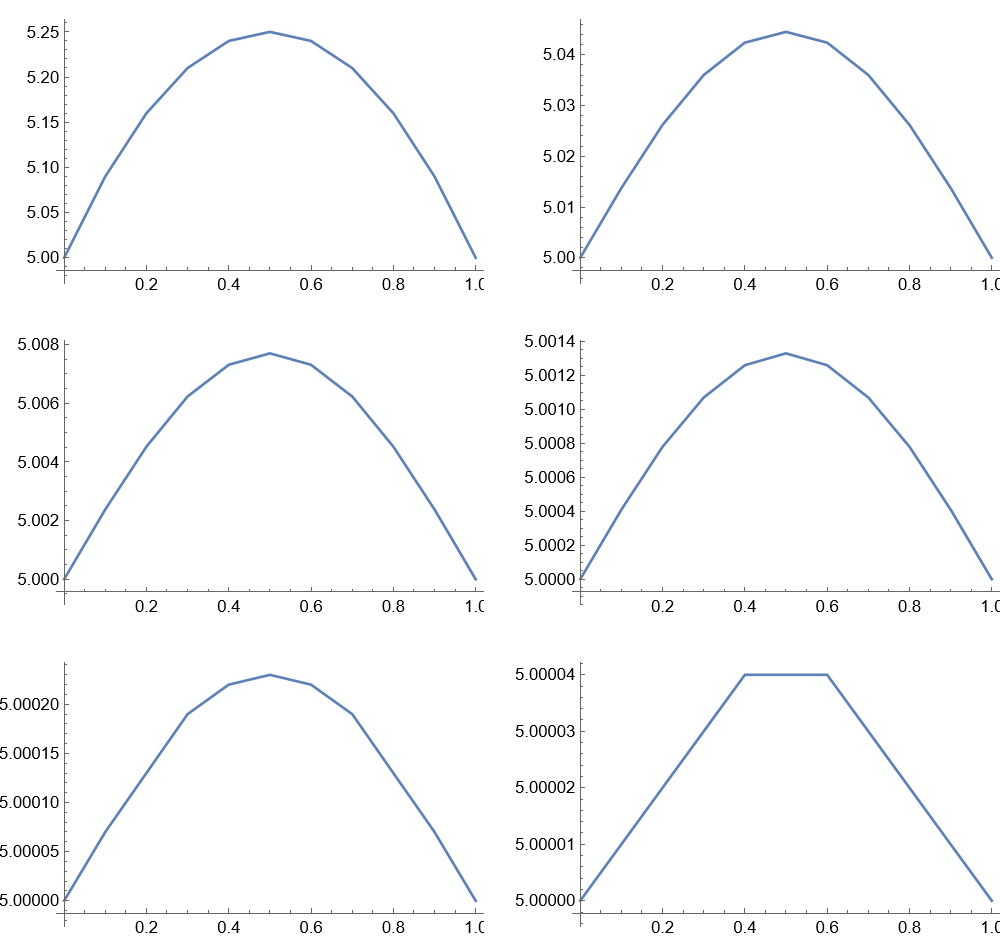
\includegraphics[width=0.9\linewidth]{with_mono}
			\caption{Иллюстрация монотонности}
			\label{with_mono}
		\end{figure}
		
		\begin{figure}[!h]
			\centering
			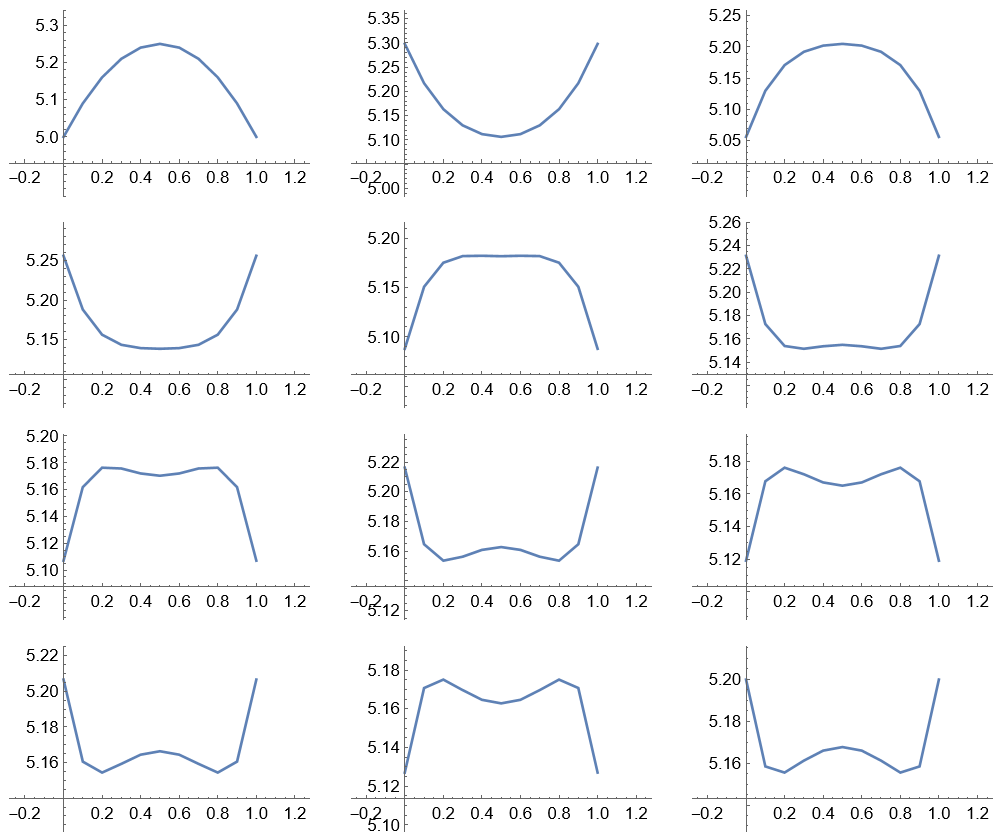
\includegraphics[width=0.9\linewidth]{without_mono}
			\caption{Иллюстрация отсутствия монотонности}
			\label{without_mono}
		\end{figure}
		
		\begin{comment}
			Если взять параметры, соответствующие указанному немонотонному случаю, то получаем следующую численную схему для нахождения значения на новом временном слое:
			\[
			y_i^{j+1} = \frac34 y_{i-1}^j -\frac12 y_i^j + \frac34 y_{i+1}^j.
			\]
			
			%В этом примере отсутствие монотонности во втором случае связано с неустойчивостью численного решения.
			
			% вроде нормальное обоснование немонотонности
			Таким образом, значение в узле на новом слое обратно пропорционально значению в этом же узле на старом слое, что и видно на графиках при сравнении соседних моментов времени. Данное поведение противоречит физическому смыслу дифференциального уравнения.
		\end{comment}
		
		\item \textit{Какие ограничения на $h,\,\tau$ и $\sigma$ накладывают условия устойчивости прогонки?}
		\smallskip
		
		Однородная консервативная разностная схема для уравнения теплопроводности:
		\begin{multline*}
			c\rho \frac{\hat y_i-y_i}{\tau}=\frac1{h}\left[\sigma\left(\hat k_{i+\frac12}\frac{\hat y_{i+1}-\hat y_i}{h}-k_{i-\frac12}\frac{\hat y_{i}-\hat y_{i-1}}{h}\right)+\right.\\
			+ \left.(1-\sigma)\left( k_{i+\frac12}\frac{y_{i+1}-y_i}{h}-k_{i-\frac12}\frac{y_{i}-y_{i-1}}{h}\right)\right]
		\end{multline*}
		
		Разностная задача решается методом прогонки:
		\begin{gather*}
			A_i \hat y_{i-1}-C_i \hat y_i+B_i \hat y_{i+1}=-F_i,\quad i=1,2,\dots,N-1,\\
			\hat y_0 = u_0,\;\hat y_N=\varkappa \hat y_{N-1}+\mu,
		\end{gather*}
		где
		\begin{gather*}
			A_i=\frac{\sigma}{h}a_i,\;	B_i=\frac{\sigma}{h}a_{i+1},\;C_i=\frac{\sigma}{h}a_i+\frac{\sigma}{h}a_{i+1}+c\rho\frac{h}{\tau},\\
			F_i=c\rho\frac{h}{\tau}y_i+(1-\sigma)(w_{i+\frac12}-w_{i-\frac12}),\\
			\varkappa = \frac{\sigma a_N/N}{c\rho h/(2\tau)+\sigma a_N/h},\\
			\mu=\frac{c\rho y_N h/(2\tau)+\sigma P(t_{j+1})+(1-\sigma)(P(t_j)-w_{N-\frac12})}{c\rho h /(2\tau)+\sigma a_N/h}.
		\end{gather*}
		\textbf{Определение.} \textbf{\textit{Метод прогонки}} называется \textbf{\textit{корректным}}, если знаменатели в формулах для прогоночных коэффициентов не обращаются в нуль, и \textbf{\textit{устойчивым}}, если все прогоночные коэффициенты $|\alpha_i|\le 1.$	
		
		\textbf{Теорема.} Пусть в трехдиагональной матрице выполнено \textbf{\textit{условие диагонального преобладания}}
		\[
		|C_i|\ge|A_i|+|B_i|,\; i=1,\dots,n,
		\]
		в котором хотя бы для одного $i$ выполнено строгое неравенство, $|C_1|>0$ и $|B_i|>0,\,i=2,\dots,n-1$. Тогда система уравнений с такой матрицей имеет решение, которое может быть получено методом прогонки. Алгоритм прогонки в указанных условиях устойчив и корректен.
		
		\[
		\left|\frac{\sigma}{h}a_i+\frac{\sigma}{h}a_{i+1}+c\rho\frac{h}{\tau}\right|\ge\left|\frac{\sigma}{h}a_i\right|+\left|\frac{\sigma}{h}a_{i+1}\right|,\;i=1,\dots,N-1.
		\]
		Условия теоремы выполнены, значит метод прогонки устойчив.
		
		Ограничения за счет граничных условий (условия I рода никак не повлияют на устойчивость прогонки, т.к. они влияют только на $F_1$ и $F_{N-1}$, которые никак не упоминаются в теореме):
		\begin{gather*}
			\varkappa \hat y_{N-1}-\hat y_N=-\mu,\; \text{где}\; A_N = \varkappa,\, C_N=1,\,F_N=\mu,\\
			|C_N|=1\ge\left|\frac{\sigma a_N/h}{c\rho h/(2\tau)+\sigma a_N/h}\right|=|A_N|,\\
			-1\le\frac{\sigma a_N/h}{c\rho h/(2\tau)+\sigma a_N/h}\le1,
		\end{gather*}
		Т.к. $c>0,\quad \rho>0,\quad h>0,\quad\tau>0,\quad0\le\sigma\le1$, получаем
		\[
		0\le\frac{\sigma a_N/h}{c\rho h/(2\tau)+\sigma a_N/h}\le1
		\]
		Таким образом, получаем, что для $0\le\sigma\le1,\, \tau>0,\,h>0$ прогонка будет устойчивой.
		При задании теплового потока на левом конце аналогично.
		
		\item \textit{В случае $K=K(u)$ чему равно количество внутренних итераций, если итерационный процесс вести до сходимости, а не обрывать после нескольких первых итераций?}
		\smallskip
		
		Возьмем пример из методического пособия.
		\begin{eqnarray*}
			& \dfrac{\partial u}{\partial t} = \dfrac{\partial}{\partial t}\left(\varkappa_0 u^\sigma \dfrac{\partial u}{\partial x}\right), \qquad x > 0, \qquad t > 0,\\
			& u(x, 0) = 0, \qquad u(0, t) = u_0 t^{1/\sigma}, \qquad u_0 = \left(\dfrac{\sigma c^2}{\varkappa_0}\right)^{1/\sigma},\\
			& \sigma = 2, \qquad \varkappa_0 = 0.5, \qquad c = 5, \qquad h = 0.2, \qquad \tau=2 \cdot 10^{-4},\\
			& L = 10, \qquad T = 1, \qquad K(u) \dfrac{\partial u}{\partial x}\Bigg|_{x = L} = 0,\\
			& \textrm{точное решение: } u(x, t) = \begin{cases}
				[\sigma c \varkappa_0^{-1}(ct-x)]^{1/\sigma}, x \le ct,\\
				0, x \ge ct.
			\end{cases}
		\end{eqnarray*}
		
		Если вести внутренний итерационный процесс до выполнения условия $||y_i^{(s+1)}\brop-y_i^{(s)}|| \le \varepsilon = 1e-9$ в евклидовой норме, то требуется от 3 до 5 итераций (рис.~\ref{iter_count}).
		
		\begin{figure}[H]
			\centering
			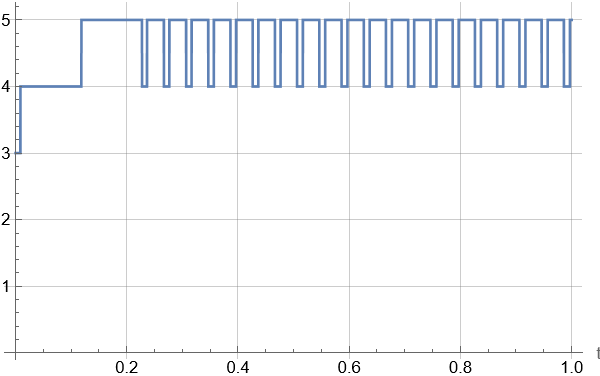
\includegraphics[width=0.8\linewidth]{iter_count}
			\caption{Количество выполненных итераций для каждого временного слоя}
			\label{iter_count}
		\end{figure}
		
		\item \textit{Для случая $K=K(u)$ предложите способы организации внутреннего итерационного процесса или алгоритмы, заменяющие его.}
		\smallskip
		
		Внутренний метод простой итерации можно представить в виде указанного ниже алгоритма.
		\begin{enumerate}
			\item Принимаем в качестве начального приближения $y_i^j$, $i = \overline{0, n}$, значения с предыдущего временного слоя $y_i^{j-1}$.
			\item Считаем значения коэффициента теплопроводности в узлах текущего временного слоя: $K_i = K(y_i^j)$, $i = \overline{0, N}$.
			\item Считаем значения $a_i = \sfrac{K(y_i^j) + K(y_{i-1}^j)}2$, $i = \overline{1, N}$.
			\item Вычисляем коэффициенты трехдиагональной СЛАУ по следующий формулам:
			\begin{eqnarray*}
				& A_i y_{i-1}^j - C_i y_i^j + B_i y_{i+1}^j = -F_i, \quad i = \overline{1, N-1}, \\
				& A_i = \dfrac{a_i}h, \quad B_i = \dfrac{a_{i+1}}h, \quad C_i = \dfrac{c\rho h}\tau + \dfrac{a_i + a_{i+1}}h, \\
				& F_i = \dfrac{c\rho h}\tau y_i^{j-1}.
			\end{eqnarray*}
			В случае граничного условия I рода на левом конце мы принимаем $y_0^j = \phi_1(t)$, $A_1 = 0$ и делаем поправку к $F_1$ на величину $\sfrac{a_1}h y_0^j$. При граничных условиях II рода в СЛАУ можно добавить строку с номером 0 вида
			\[
			- y_0^j + \varkappa y_1^j = - \nu, \quad \varkappa = \frac{a_1/h}{c\rho h/(2\tau) +a_1 h}, \quad \nu = \frac{c\rho h y_0^{j-1} + P(t_j)}{c\rho h/(2\tau) +a_1 h}.
			\]
			Аналогично для условий I и II рода на правом конце.
			\item Используя метод прогонки, находим новое приближение $y_i^j$;
			\item Если не было выполнено нужно количество итераций внутреннего метода, то переходим обратно к пункту (b), иначе переходим на следующий временной слой.
		\end{enumerate}
		
		Также вместо метода простой итерации можно использовать метод Ньютона. Для систем нелинейных уравнений вида $F(x) = 0$ его итерационная формула записывается как
		\[
		F'(x^k) (x-x^k) = -F(x^k).
		\]
		
		Для неявной схемы уравнения теплопроводности при граничных условиях I рода
		\begin{eqnarray*}
			& F_i(y) = \sfrac{a(y_i)}h y_{i-1} - \left(\sfrac{c \rho h}\tau + \sfrac{a(y_{i+1}) + a(y_i)}h\right) y_i + \sfrac{a(y_{i+1})}h y_{i+1} - \sfrac{c\rho h}\tau y_i^{j-1}, \\
			& a(y_k) = \sfrac{K(y_k) + K(y_{k-1})}2, \quad i = \overline{1, N-1}.
		\end{eqnarray*}
		
		Как и в случае метода простой итерации при заданных границах I рода $y_0$ и $y_N$ считаются известными и не входят в систему уравнений как переменные, требующие определения.
		
		Заметим, что т.к. в $i$-ом уравнении участвуют только переменные $y_{i-1}$, $y_i$ и $y_{i+1}$, то матрица Якоби решаемой системы будет трехдиагональной. Таким образом, для решения СЛАУ итерационной формулы можно также применять метод прогонки. Распишем коэффициенты указанной матрицы для $a(y_k) \brop= \sfrac{K(y_k) + K(y_{k-1})}2$:
		\begin{eqnarray*}
			& \dfrac{\partial F_i}{\partial y_{i-1}} = \dfrac1h \dfrac{\partial}{\partial y_{i-1}} (a(y_i) y_{i-1}) - \dfrac1h \dfrac{\partial a(y_i)}{\partial y_{i-1}} y_i, \quad \dfrac{\partial a(y_i)}{\partial y_{i-1}} = \dfrac12 K'(y_{i-1}),\\
			& \dfrac{\partial F_i}{\partial y_{i-1}} = \dfrac1{2h} K'(y_{i-1}) (y_{i-1} - y_i) + \dfrac{a(y_i)}h, \\
			& \dfrac{\partial F_i}{\partial y_{i+1}} = \dfrac1{2h} K'(y_{i+1}) (y_{i+1} - y_i) + \dfrac{a(y_{i+1})}h,\\
			& \dfrac{\partial F_i}{\partial y_i} = \dfrac{K'(y_i)}{2h} (y_{i-1} + y_{i+1}) - \dfrac{c\rho h}\tau - \dfrac{a(y_{i+1}) + a(y_i)}h - \dfrac{K'(y_i)}h y_i,\\
			& \dfrac{\partial F_i}{\partial y_i} = \dfrac{K'(y_i)}{2h} (y_{i-1} -2y_i + y_{i+1}) - \dfrac{c\rho h}\tau - \dfrac{a(y_{i+1}) + a(y_i)}h.
		\end{eqnarray*}
		
	\end{enumerate}
	\newpage
	\section{Результаты}
	
	\subsection{Проверка консервативности}
	
	\hphantom{1}\\[-2.5cm]
	
	\begin{eqnarray*}
		& K \equiv 3, \quad c\rho = 1, \quad L = 20, \quad T = 1, \quad h =  0.55, \quad \tau = 0.005,\\
		& -K(u) \dfrac{\partial u}{\partial x}\Bigg|_{x=0} = K(u) \dfrac{\partial u}{\partial x}\Bigg|_{x=L} = 0.
	\end{eqnarray*}
	
	При $\sigma = 0$, 0.5 и 1 график разности $\Big|\sfrac h2 y_0^{j+1} + h \sum_{i=1}^{N-1} y_i^{j+1} + \sfrac h2 y_N^{j+1} - \sfrac h2 y_0^j - h \sum_{i=1}^{N-1} y_i^j \brop- \sfrac h2 y_N^j\Big|$ представлен на рис.~\ref{diff_0}, \ref{diff_0.5} и \ref{diff_1} соответственно.
	
	\begin{figure}[H]
		\centering
		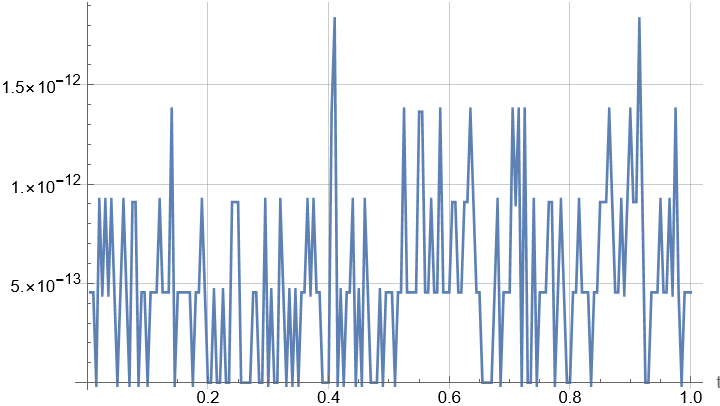
\includegraphics[width=0.8\linewidth]{diff_0}
		\caption{График разности при $\sigma = 0$}
		\label{diff_0}
	\end{figure}
	
	\begin{figure}[H]
		\centering
		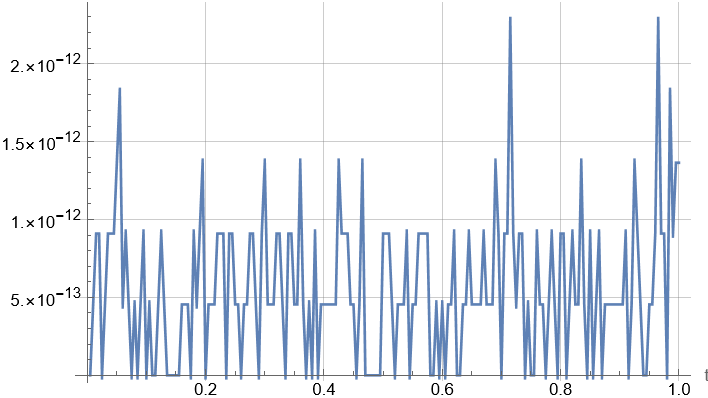
\includegraphics[width=0.8\linewidth]{diff_0.5}
		\caption{График разности при $\sigma = 0.5$}
		\label{diff_0.5}
	\end{figure}
	
	\begin{figure}[H]
		\centering
		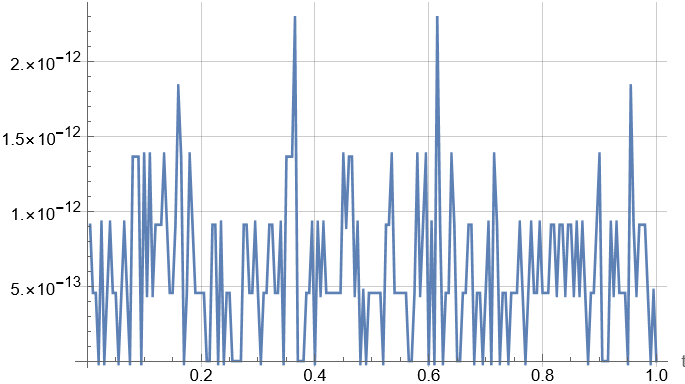
\includegraphics[width=0.8\linewidth]{diff_1}
		\caption{График разности при $\sigma = 1$}
		\label{diff_1}
	\end{figure}
	
	\subsection{График погрешности в случае K(u)}
	
	\hphantom{1}\\[-2.5cm]
	
	\begin{eqnarray*}
		& \dfrac{\partial u}{\partial t} = \dfrac{\partial}{\partial t}\left(\varkappa_0 u^\sigma \dfrac{\partial u}{\partial x}\right), \qquad x > 0, \qquad t > 0,\\
		& u(x, 0) = 0, \qquad u(0, t) = u_0 t^{1/\sigma}, \qquad u_0 = \left(\dfrac{\sigma c^2}{\varkappa_0}\right)^{1/\sigma},\\
		& \sigma = 2, \qquad \varkappa_0 = 0.5, \qquad c = 5, \qquad h = 0.2, \qquad \tau=2 \cdot 10^{-4},\\
		& L = 10, \qquad T = 1, \qquad K(u) \dfrac{\partial u}{\partial x}\Bigg|_{x = L} = 0,\\
		& \textrm{точное решение: } u(x, t) = \begin{cases}
			[\sigma c \varkappa_0^{-1}(ct-x)]^{1/\sigma}, x \le ct,\\
			0, x \ge ct.
		\end{cases}
	\end{eqnarray*}
	
	График погрешности представлен на рис.~\ref{error_u}.
	% TODO Вы получили очень необычный график. Можете, пожалуйста, объяснить, почему он так выглядит? И должна ли возникать такая картинка? (расписать получше)
	Такое поведение графика можно объяснить тем, что при $x = ct$ производная точного решения терпит разрыв. Получаем, что в точках, близких к $x = ct$, погрешность аппроксимации резко возрастает.
	
	\begin{figure}[h!]
		\centering
		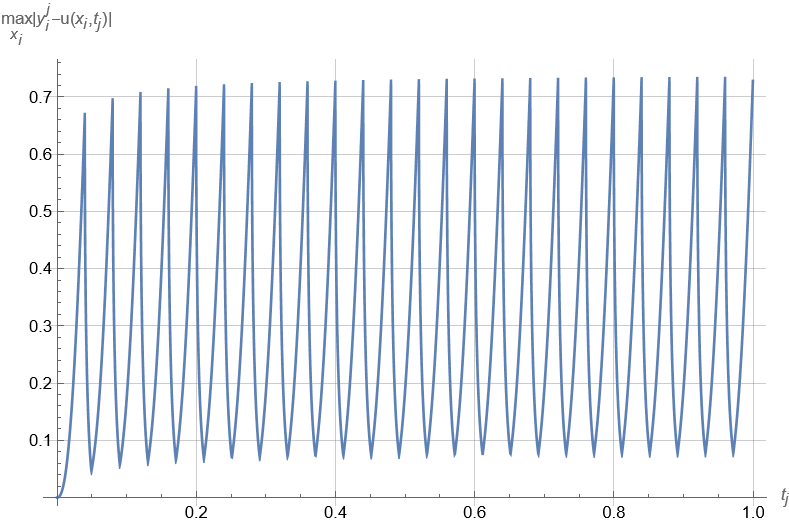
\includegraphics[width=0.85\linewidth]{error_u}
		\caption{График погрешности численного решения в случае $K(u)$}
		\label{error_u}
	\end{figure}
	
	\subsection{Оценка порядка сходимости}
	%	\[
	%	\mathbf{q=\frac12}
	%	\]
	\begin{table}[H]
		\caption{Порядок сходимости ($\sigma=0$), пример неустойчив}
		\centering
		\begin{tabular}{|c|c|c|c|}\hline
			$\tau,\;h$ & AbsErr($\tau,\,h$) & $\Delta$ & $\log_q \Delta$\\ 
			\hline
			0.5, 0.5&&&\\
			\hline
			---, ---&&&\\
			\hline
			---, ---&&&\\
			\hline
			---, ---&&&\\
			\hline
			---, ---&&&\\
			\hline
			---, ---&&&\\
			\hline
		\end{tabular}
	\end{table}
	
	\begin{table}[H]
		\caption{Порядок сходимости ($\sigma=1$)}
		\centering
		\begin{tabular}{|c|c|c|c|}\hline
			$\tau,\;h$ & AbsErr($\tau,\,h$) & $\Delta$ & $\log_q \Delta$\\ 
			\hline
			0.05, 0.5&0. 0.014611&---&---\\
			\hline
			0.0125, 0.25& 0.00390149& 0.267024& 1.90496\\
			\hline
			0.003125, 0.125&0.000990189&0.253798&1.97825\\
			\hline
			0.00078125, 0.0625& 0.000248762&0.251227&1.99728\\
			\hline
			0.000195313, 0.03125& 6.23079e-05& 0.250472&1.99728\\
			\hline
			4.88281e-05, 0.015625&1.57214e-05&0.252317&1.98669\\
			\hline
		\end{tabular}
	\end{table}
	
	\begin{table}[H]
		\caption{Порядок сходимости ($\sigma=\frac12$)}
		\centering
		\begin{tabular}{|c|c|c|c|}\hline
			$\tau,\;h$ & AbsErr($\tau,\,h$) & $\Delta$ & $\log_q \Delta$\\ 
			\hline
			0.05, 0.5&0.  0.00678697&---&---\\
			\hline
			0.0125, 0.25& 0.00178249& 0.262634& 1.92888\\
			\hline
			0.003125, 0.125&0.000451189& 0.253123&1.98209\\
			\hline
			0.00078125, 0.0625&  0.000113204&0.250902&1.9948\\
			\hline
			0.000195313, 0.03125&  2.83079e-05&0.250061&1.99965\\
			\hline
			4.88281e-05, 0.015625& 7.52347e-06&0.265773& 1.91173\\
			\hline
		\end{tabular}
	\end{table}
	
	
	\clearpage
	\begin{thebibliography}{1}
		\bibitem{galanin} \textit{Галанин М.П., Савенков Е.Б.} Методы численного анализа математических\\ моделей. М.: Изд-во МГТУ им. Н.Э. Баумана,	2010. 592 с.
		\bibitem{kalitkin} \textit{Калиткин Н.Н.} Численные методы. М.: Наука, 1978. 512 с.
		\bibitem{godunov} \textit{Годунов С.К., Рябенький В.С.} Разностные схемы (введение в теорию). М.: Наука, 1977. 440 с.
		
		
	\end{thebibliography}
	
	
\end{document}
